\documentclass[a4paper,12pt,leqno]{article}

\usepackage[utf8]{inputenc}
\usepackage[width=15cm,height=21cm]{geometry}
\usepackage{amsmath,amsfonts,amssymb,amsthm}
\usepackage{mathrsfs}
\usepackage[hidelinks,pdfusetitle]{hyperref}
\usepackage[capitalise]{cleveref}
\usepackage{bbm}

\usepackage{tikz}
\usetikzlibrary{arrows.meta}

\usepackage{enumitem}

\usepackage{sectsty}
\sectionfont{\fontsize{12}{15}\selectfont}

% Figures with no caption
\usepackage{caption}
\DeclareCaptionFormat{empty}{Fig.#1}
\renewcommand*\figurename{}
\captionsetup{format=empty}

\numberwithin{equation}{section}

% Used to rename "Problem A"
\newtheorem{innerproblem}{}
\newenvironment{thm}[1]
{\renewcommand\theinnerproblem{#1}\innerproblem}
{\endinnerproblem}

\newcommand{\dd}{\mathop{}\!\mathrm{d}}

\crefname{thm}{Theorem}{Theorems}

\title{On a Unified Theory \\
of Boundary Value Problems \\
for Elliptic-Parabolic Equations \\
of Second Order}
\author{Gaetano Fichera}
\date{}

\newcommand{\lub}[1]{\underset{#1}{\operatorname{l.u.b.}}}
\newcommand{\ovdir}{\overline{\Sigma_{D}^{(3)}}}

\begin{document}

\maketitle

The present lecture is concerned with the theory of boundary value problems for linear partial differential equations of second order. 
It consists of a proposal for a unified theory of boundary value problems for second order linear equations of elliptic-parabolic type, including the classical cases of totally elliptic equations, heat equation, and first order equations.

The theory does not claim to be complete at this time. 
Nevertheless it opens, in my opinion, many attractive fields for further research and, therefore, the results obtained up to the present time deserve to be expounded here.

The first results of this theory were obtained by the writer in 1956
\cite{4}. 
A more complete treatment can be found in the mimeographed notes containing the lectures the writer delivered at the Istituto Italiano di Alta Matematica in Rome in 1957 \cite{5}.

In 1958, K.\ O.\ Friedrichs published a paper \cite{7} on boundary value problems for linear differential equations independent of type. 
The Friedrichs theory covers equations that may be hyperbolic in one subregion of the domain where the problem is considered and elliptic in a different subregion. 
However, it does not seem possible to include in the class of equations considered by Friedrichs every elliptic-parabolic equation, since Friedrichs assumes a symmetry condition, that is not needed in the present treatment.
A comparison between the Friedrichs theory and the present one would be -- in the opinion of the writer -- very interesting.

\section{Hypotheses and statement of the general boundary value problem for second order linear elliptic-parabolic equations}

Let us denote by $X^{(r)}$ the $r$-dimensional real Cartesian space.
Let $x \equiv\left(x_{1}, \ldots, x_{r}\right)$ be a point in $X^{(r)}$ and $B$ a connected open set in $X^{(r)}$.
A function is said to belong to $C^{m}(B)$ ($m$ nonnegative integer) if it is continuous in $B$ together with its partial derivatives of order $h \leq m$. Let $a^{i j}(x)$ ($i, j=1, \ldots, r$), $b^i(x)$ ($i=1, \ldots, r)$, $c(x)$ be real functions of $C^{2}(B)$, $C^{1}(B)$, $C^{0}(B)$ respectively.

We shall consider the following second order linear differential operator:
$$L(u) \equiv a^{i j} u_{x_{i} x_{j}}+b^{i} u_{x_{i}}+c u
\quad {}(\ref{note:1})
\quad\quad
\left(a^{ij} \equiv a^{ji}\right)$$
and suppose that for any $x \in B$ the quadratic form $a^{i j}(x) \lambda_{i} \lambda_{j}$ is positive definite or semi-definite, that is to say that $L$ is a positive elliptic-parabolic operator in $B$. 
The case that perhaps for some points of $B$, $a^{i j}(x) \lambda_{i} \lambda_{j} \equiv 0$ is not excluded.

This means that in some subset of $B$ -- possibly coinciding with $B$ -- the differential operator might degenerate to a first order operator.

Let $A$ be a bounded open set contained in $B$ such that its boundary $\Sigma$ coincides with the boundary of its closure $\bar{A}$.

In order to state the exact hypotheses to be assumed on $\Sigma$, we shall define first what we mean by a \emph{regular $(r-1)$-cell} in $X^{(r)}$.

Let $x=x(t)$ be a function, defined in a closed domain $D$ of the Cartesian $(r-1)$-space and with range in $X^{(r)}$, satisfying the following conditions: (a.) $D$ is homeomorphic to an $(r-1)$-sphere, (b.) $x(t)$ maps $D$ one-to-one onto a subet of $X^{(r)}$, (c.) the rank of the Jacobian matrix $\partial(x)/\partial(t)$ is $r-1$ at any point of $D$, (d.) the $(r-1)$-Lebesgue measure of the boundary of $D$ is zero. 

The range $\Sigma_{0}$ of $x(t)$ is an \emph{$(r-1)$-regular cell of $\quad X^{(r)}$}. 
The image of the boundary of $D$ is called \emph{the border} of $\Sigma_{0}$.

We shall suppose that $\Sigma$ can be decomposed in a finite number of regular $(r-1)-$ cells: $\Sigma=\Sigma_{1} \cup \ldots \cup \Sigma_{m}$ such that any two of them have at most points of their borders in common.

In addition we shall suppose that the Green-Gauss identity, that transforms an $r$-integral over A into an $(r-1)$-integral over $\Sigma$, can be applied to $A \cup \Sigma$.

Let us denote by $\Sigma_{h}'$ the subset of $\Sigma_{h} $ ($h=1, \ldots, m$) such that at any point $x$ of $\Sigma'_h$ the tangent hyperplane to $\Sigma_{h}$ is characteristic with respect to the operator L. This means that the direction cosines $n_{1}, \ldots, n_{r}$ of the normal to $\Sigma_{h}$ at $x$ satisfy the equation:
$A^{ij}(x) n_{i} n_{j}=0$. 
At any point $x$ of $\Sigma_{h}$, not lying on the border of $\Sigma_h$, the function
\begin{equation*}
	b(x)=\left(b^i-a_{x_{j}}^{i j}\right) n_i,
\end{equation*}
is well defined, where $n_{1}, \ldots, n_{r}$ are the direction cosines of the inner normal to $A$ at the point $x$ of $\Sigma_{h}$.

For any fixed $h$ we can extend the definition of $b(x)$ by continuity over all $\Sigma_{h}$~(\ref{note:2}). 
Let $\Sigma_{h}^{(1)}$ be the subset of $\Sigma_{h}'$ defined by the condition $b(x) \geq 0$.
Let us set:
\begin{equation*}
	\begin{aligned}
		&\Sigma^{(1)}=\Sigma_{1}^{(1)} \cup \Sigma_{2}^{(1)} \cup \ldots \cup \Sigma_{m}^{(1)} \\
		&\Sigma^{(2)}=\left(\Sigma'_{1} \cup \Sigma'_{2} \cup \ldots \cup \Sigma_{m}'\right)-\Sigma^{(1)} \\
		&\Sigma^{(3)}=\Sigma-\left(\Sigma^{(1)} \cup \Sigma^{(2)}\right) .
	\end{aligned}
\end{equation*}

The set $\Sigma$ is decomposed in three disjoint subsets $\Sigma^{(1)}, \Sigma^{(2)}$, $\Sigma^{(3)} \cdot$ It must be observed that someone of these sets might be empty.

Let $\Sigma_{D}^{(3)}$ and $\Sigma_{N}^{(3)}$ be two disjoint sets such that
\begin{equation*}
	\Sigma^{(3)}=\Sigma_{D}^{(3)} \cup \Sigma_{N}^{(3)}.
\end{equation*}
The set $\Sigma_{D}^{(3)}$ or $\Sigma_{N}^{(3)}$ may be assumed to be empty. 
Of course both these sets are empty when $\Sigma^{(3)}$ is empty.

Let $f(x)$, $g(x)$, $h(x)$ be given functions defined respectively on $A$, on $\Sigma^{(2)} \cup \Sigma_{D}^{(3)}$ and on $\Sigma_{N}^{(3)}$.

The boundary value problem that we shall consider for a general elliptic-parabolic equation is the following:
\begin{equation} \label{eq:1.1}
	\boxed{
	\begin{aligned}
		&L(u)=f && \quad \text{in } A,\\
		&u=g && \quad \text{on } \Sigma^{(2)}\cup\Sigma_D^{(3)},\\
		&A^{i j}(x) u_{x_{i}} n_{j}=h && \quad \text{on } \Sigma_N^{(3)}.
	\end{aligned}
	}
\end{equation}

\section{Particular cases and examples}
\label{sec:2}

Let us suppose $a^{ij}(x)\lambda_i\lambda_j$ positive definite in any point of $B$, that is to say that $L$ is a totally elliptic operator.
In this particular case $\Sigma^{(1)}$ and $\Sigma^{(2)}$ are both empty. 
If $\Sigma_{N}^{(3)}$ is assumed empty, the boundary value problem \eqref{eq:1.1} is the classical Dirichlet problem. 
If $\Sigma_{\mathrm{D}}^{(3)}$ is empty, we have the Neumann problem for a general elliptic operator. 
In the case that $\Sigma_{D}^{(3)}$ and $\Sigma_{N}^{(3)}$ are not empty, problem \eqref{eq:1.1} reduces to the mixed Dirichlet-Neumann boundary value problem for an elliptic operator.
Let us now assume:
\begin{equation*}
	L(u) \equiv L_{0}(u)-u_{x_{r}}
\end{equation*}
where $L_{0}$ is an elliptic operator in the $r-1$ variables: $x_{1}, \ldots, x_{r-1}$.
In this case $L$ is the well known parabolic heat equation operator.
$\Sigma^{(1)}$ is the part of $\Sigma$ where the inner normal $n$ is parallel, and opposite in direction to the $x_{r}$-axis (hatched line in \cref{fig:1}), $\Sigma^{(2)}$ the part of $\Sigma$ where $n$ is parallel to the $x_{r}$-axis and oriented as this axis. $\Sigma^{(3)}$ is the part of the boundary where $n$ and $x_{r}$ form an angle different from~$0$ and~$\pi$.

\begin{figure}
	\centering
	\begin{tikzpicture}[>=Stealth]
		\draw[->] (-1,0) -- (6,0) node[anchor=north] {$x_r=0$};
		\draw[->] (0,-1) -- (0,6) node[anchor=east] {$x_r$};
		\draw[very thick] (1,1.5) -- (3,1.5) node[anchor=north] {$\Sigma^{(2)}$} -- (5,1.5);
		\draw[very thick, dashed] (1,4.5) -- (3,4.5) node[anchor=south] {$\Sigma^{(4)}$} -- (5,4.5);
		\draw[very thick] (1,1.5) .. controls (2,3) and (0,3.5) .. (1,4.5);
		\node[left] at (1,3) {$\Sigma^{(3)}$};
		\draw[very thick] (5,1.5) .. controls (4,2) and (6.5,3.5) .. (5,4.5);
		\node[right] at (5.4,3) {$\Sigma^{(3)}$};
	\end{tikzpicture}
	\caption{}
	\label{fig:1}
\end{figure}

Let us consider the more general parabolic operator:
\begin{equation*}
	L(u) \equiv L_{0}(u)-b^{r}(x) u_{x_{r}}
\end{equation*}
where $L_{0}$ is defined as above (elliptic operator in the variables $x_{1}, \ldots, x_{r-1}$) and $b^{r}(x)$ is an arbitrary function, not necessarily of fixed sign, in $A \cup \Sigma$. 
We do not exclude that the coefficients of $L_{0}$ may depend also on the variable $x_{r}$.

Let $W^{+}$ ($W^{-}$) be the part (possibly empty) of $\Sigma$ where the inner normal $n$ is parallel and equiverse (opposite) to the $x_{r}$-axis.
$W^+_1$ ($W^-_1$) be the subset of $W^+$ ($W^-$) where $b_{r}(x) \geq 0$ ($b_{r}(x) \leq 0$) and $W^+_2$ ($W^-_2$) the remaining part. 
We have:
$\Sigma^{(1)} \supset W^{+}_{1} \cup W_{1}^{-}$; $\Sigma^{(2)} \supset W^{+}_{2} \cup W^{-}_{2}$.
It is easy to see how to distribute the points of $\Sigma$ where the tangent hyperplane is not defined.
As an example consider the parabolic equation
\begin{equation*}
	\frac{\partial^{2} u}{\partial x_{1}^{2}}-\sin x_{1} \frac{\partial u}{\partial x_{2}}=f\left(x_{1}, x_{2}\right),
\end{equation*}
in the domain indicated in \cref{fig:2}.

\begin{figure}
	\centering
	\begin{tikzpicture}[>=Stealth]
		\draw[->] (-1,0) -- (13,0) node[anchor=north] {$x_1$};
		\draw[->] (0,-2) -- (0,7) node[anchor=east] {$x_2$};
		\node[below left] at (0,0) {$0$};
		
		\draw[very thick] (0,0) -- (2.5,0) node[anchor=north] {$\Sigma^{(2)}$} -- (5,0);
		\draw[very thick] (5,0.1) -- (5,-0.1) node[anchor=north] {$\pi$};
		\draw[very thick, dashed] (5,0) -- (7.5,0) node[anchor=south] {$\Sigma^{(1)}$} -- (10,0);
		\draw[very thick] (10,0.1) -- (10,-0.1) node[anchor=north] {$2\pi$};
		\draw[very thick] (10,0) -- (12,0) node[anchor=north] {$a$};
		
		\draw[very thick, dashed] (0,5) -- (2.5,5) node[anchor=north] {$\Sigma^{(1)}$} -- (5,5);
		\draw[very thick] (5,5) -- (7.5,5) node[anchor=south] {$\Sigma^{(2)}$} -- (10,5);
		\draw[very thick] (5,5.1) -- (5,4.9);
		\draw[very thick] (10,5.1) -- (10,4.9);		
		\draw[very thick, dashed] (10,5) -- (10.5,5) node[anchor=north] {$\Sigma^{(1)}$} -- (11.5,5);
		
		\draw[very thick] (0,0) 
		.. controls ++(0:0) and ++(90:-1) .. (-1,1.5)
		.. controls ++(90:1) and ++(90:-0.5) .. (-0.2,3)
		.. controls ++(90:0.5) and ++(90:-0.5) .. (-0.5,4)
		.. controls ++(90:0.5) and ++(0:0) .. (0,5);
		\node[left] at (-0.6,3) {$\Sigma^{(3)}$};
		
		\draw[very thick] (12,0) 
		.. controls ++(0:0) and ++(90:-1) .. (13,1.5)
		.. controls ++(90:1) and ++(90:-1) .. (11,4)
		.. controls ++(90:1) and ++(0:0) .. (11.5,5);
		\node[right] at (12,3) {$\Sigma^{(3)}$};
	\end{tikzpicture}
	\caption{}
	\label{fig:2}
\end{figure}

The hatched line denotes the part $\Sigma^{(1)}$ of $\Sigma$ where one must not prescribe any boundary condition.

As very simple and elementary examples consider the two first order equations:
\begin{equation*}
	u_{x_{1}}+c(x) u=f(x), \quad x_{1} u_{x_{1}}+x_{2} u_{x_{2}}+c(x) u=f(x)
\end{equation*}
In \cref{fig:3} and \cref{fig:4} the parts $\Sigma^{(1)}$ and $\Sigma^{(2)}$ of $\Sigma$ are, respectively, shown ($\Sigma^{(1)} \equiv$ hatched line, $\Sigma^{(2)} \equiv$ continuous line).

\begin{figure}
	\centering
	\begin{minipage}{.49\textwidth}
		\centering
		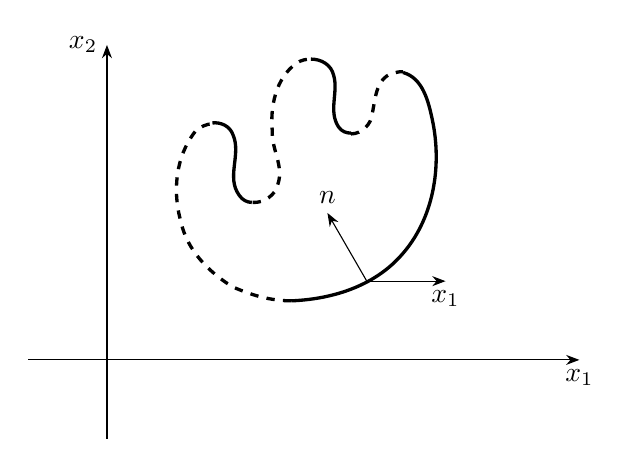
\begin{tikzpicture}[>=Stealth]
			\draw[->] (0,-5) -- (7,-5) node[anchor=north] {$x_1$};
			\draw[->] (1,-6) -- (1,-1) node[anchor=east] {$x_2$};
			
			\draw[->] (4.3,-4) -- ++(0:10mm) node[anchor=north] {$x_1$};
			\draw[->] (4.3,-4) -- ++(120:10mm) node[anchor=south] {$n$};
			
			\draw [very thick, dashed] (33.4mm,-42.5mm)
			.. controls ++(-1.7mm,0.0mm) and ++(1.6mm,-0.5mm) .. ++(-4.9mm,0.8mm)
			.. controls ++(-0.9mm,0.3mm) and ++(0.9mm,-0.4mm) .. ++(-2.6mm,1.0mm)
			-- ++(0.0mm,0.0mm)
			.. controls ++(-3.0mm,1.9mm) and ++(0.8mm,-3.6mm) .. ++(-6.5mm,8.2mm)
			.. controls ++(-1.1mm,3.9mm) and ++(-2.5mm,-3.2mm) .. ++(1.8mm,11.5mm)
			.. controls ++(0.6mm,0.6mm) and ++(-0.8mm,0.0mm) .. ++(2.3mm,1.0mm)
			;
			\draw [very thick] (47.6mm,-13.5mm)
			.. controls ++(2.5mm,-0.7mm) and ++(-0.5mm,2.3mm) .. ++(3.7mm,-5.9mm)
			.. controls ++(1.3mm,-6.0mm) and ++(4.2mm,4.6mm) .. ++(-4.0mm,-17.4mm)
			.. controls ++(-3.5mm,-3.9mm) and ++(5.1mm,0.2mm) .. ++(-13.9mm,-5.7mm)
			;
			\draw [very thick, dashed] (41.0mm,-21.3mm)
			.. controls ++(1.3mm,0.0mm) and ++(-0.1mm,-1.4mm) .. ++(2.7mm,2.6mm)
			.. controls ++(0.4mm,2.0mm) and ++(-2.5mm,-0.4mm) .. ++(3.0mm,5.2mm)
			.. controls ++(0.3mm,0.1mm) and ++(-0.3mm,0.0mm) .. ++(0.9mm,0.1mm)
			;
			\draw [very thick] (35.9mm,-11.8mm)
			.. controls ++(1.3mm,0.0mm) and ++(-0.3mm,1.4mm) .. ++(2.9mm,-2.1mm)
			.. controls ++(0.6mm,-2.1mm) and ++(-1.3mm,2.0mm) .. ++(0.6mm,-6.5mm)
			.. controls ++(0.4mm,-0.6mm) and ++(-0.6mm,0.0mm) .. ++(1.6mm,-0.8mm)
			;
			\draw [very thick, dashed] (28.5mm,-30.0mm)
			.. controls ++(1.4mm,-0.1mm) and ++(-0.3mm,-1.4mm) .. ++(3.2mm,2.3mm)
			.. controls ++(0.8mm,2.3mm) and ++(-0.1mm,-2.3mm) .. ++(-0.7mm,6.7mm)
			.. controls ++(-0.3mm,3.1mm) and ++(-2.7mm,-1.9mm) .. ++(3.1mm,8.7mm)
			.. controls ++(0.6mm,0.4mm) and ++(-0.7mm,-0.0mm) .. ++(1.9mm,0.5mm)
			;
			\draw [very thick] (23.4mm,-19.9mm)
			.. controls ++(1.1mm,0.1mm) and ++(-0.4mm,1.1mm) .. ++(2.6mm,-1.5mm)
			.. controls ++(1.1mm,-2.5mm) and ++(-1.7mm,2.3mm) .. ++(0.8mm,-7.7mm)
			.. controls ++(0.4mm,-0.6mm) and ++(-0.6mm,-0.0mm) .. ++(1.6mm,-0.9mm)
			;
		\end{tikzpicture}
		\captionof{figure}{}
		\label{fig:3}
	\end{minipage}
	\begin{minipage}{.49\textwidth}
		\centering
		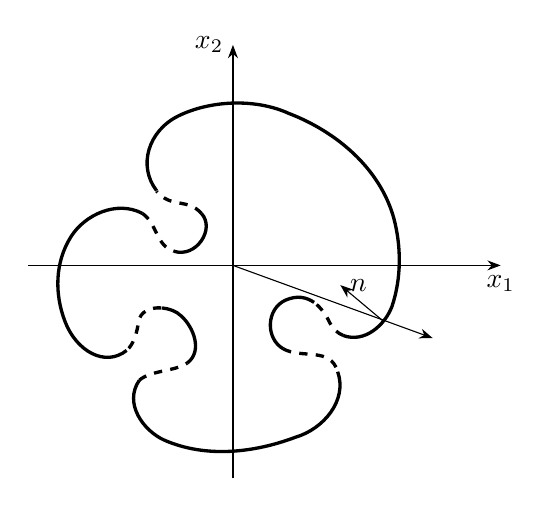
\begin{tikzpicture}[>=Stealth]
			\draw[->] (1,-2.8) -- (7,-2.8) node[anchor=north] {$x_1$};
			\draw[->] (3.6,-5.5) -- (3.6,0) node[anchor=east] {$x_2$};
			
			\draw[->] (3.6,-2.8) -- ++(-20:27mm);
			\draw[->] (5.5,-3.5) -- ++(140:7mm) node[anchor=west] {$n$};
			
			\draw [very thick] (26.3mm,-18.5mm)
			.. controls ++(-2.4mm,3.1mm) and ++(-3.9mm,-1.9mm) .. ++(2.8mm,9.5mm)
			.. controls ++(3.9mm,1.9mm) and ++(-4.4mm,2.0mm) .. ++(14.0mm,0.3mm)
			.. controls ++(6.0mm,-2.3mm) and ++(-1.8mm,6.3mm) .. ++(13.3mm,-13.2mm)
			.. controls ++(1.0mm,-3.7mm) and ++(1.2mm,3.6mm) .. ++(-0.2mm,-11.3mm)
			.. controls ++(-0.9mm,-2.4mm) and ++(2.7mm,-1.0mm) .. ++(-6.2mm,-3.7mm)
			;
			\draw [very thick, dashed] (32.0mm,-21.4mm)
			.. controls ++(-1.8mm,2.0mm) and ++(1.9mm,-2.2mm) .. ++(-5.7mm,2.8mm)
			;
			\draw [very thick] (28.5mm,-26.2mm)
			.. controls ++(2.8mm,-0.9mm) and ++(1.8mm,-2.0mm) .. ++(3.5mm,4.8mm)
			;
			\draw [very thick, dashed] (24.5mm,-21.4mm)
			.. controls ++(1.9mm,-1.3mm) and ++(-2.3mm,0.7mm) .. ++(4.0mm,-4.8mm)
			;
			\draw [very thick] (22.5mm,-38.8mm)
			.. controls ++(-2.8mm,-2.2mm) and ++(1.4mm,-3.6mm) .. ++(-7.8mm,3.6mm)
			.. controls ++(-1.4mm,3.6mm) and ++(-2.0mm,-3.2mm) .. ++(0.7mm,10.8mm)
			.. controls ++(1.8mm,2.9mm) and ++(-3.2mm,1.7mm) .. ++(9.1mm,3.0mm)
			;
			\draw [very thick, dashed] (26.9mm,-33.4mm)
			.. controls ++(-1.3mm,0.1mm) and ++(0.2mm,1.4mm) .. ++(-2.9mm,-1.8mm)
			.. controls ++(-0.2mm,-1.4mm) and ++(0.9mm,0.8mm) .. ++(-1.5mm,-3.6mm)
			;
			\draw [very thick] (30.2mm,-40.4mm)
			.. controls ++(2.0mm,1.5mm) and ++(1.6mm,-1.4mm) .. ++(-0.8mm,6.0mm)
			.. controls ++(-0.6mm,0.6mm) and ++(0.9mm,-0.1mm) .. ++(-2.4mm,1.0mm)
			;
			\draw [very thick, dashed] (24.1mm,-42.6mm)
			.. controls ++(1.4mm,1.3mm) and ++(-1.6mm,-1.1mm) .. ++(6.1mm,2.2mm)
			;
			\draw [very thick] (49.3mm,-41.5mm)
			.. controls ++(1.3mm,-3.7mm) and ++(3.4mm,1.0mm) .. ++(-5.3mm,-8.3mm)
			.. controls ++(-5.3mm,-2.0mm) and ++(5.3mm,-2.3mm) .. ++(-16.7mm,-0.4mm)
			.. controls ++(-2.7mm,1.2mm) and ++(-2.0mm,-2.9mm) .. ++(-3.2mm,7.6mm)
			;
			\draw [very thick, dashed] (42.4mm,-38.6mm)
			.. controls ++(2.3mm,-1.3mm) and ++(-0.9mm,3.2mm) .. ++(6.9mm,-2.9mm)
			;
			\draw [very thick] (46.3mm,-32.7mm)
			.. controls ++(-1.0mm,0.7mm) and ++(1.4mm,0.6mm) .. ++(-3.6mm,0.3mm)
			.. controls ++(-2.5mm,-1.1mm) and ++(-2.3mm,1.3mm) .. ++(-0.3mm,-6.2mm)
			;
			\draw [very thick, dashed] (50.0mm,-36.9mm)
			.. controls ++(-0.7mm,0.3mm) and ++(0.4mm,-0.8mm) .. ++(-1.7mm,1.6mm)
			.. controls ++(-0.5mm,1.1mm) and ++(0.8mm,-0.6mm) .. ++(-2.0mm,2.6mm)
			;
		\end{tikzpicture}
		\captionof{figure}{}
		\label{fig:4}
	\end{minipage}
\end{figure}

As a more interesting example consider the first order equation,
\begin{equation*}
	b_{1} u_{x_{1}}+b_{2} u_{x_{2}}+c u=f \text {, }
\end{equation*}
in the interval $-a_{1} \leq x_{1} \leq a_{1}$, $-a_{2} \leq x_{2} \leq a_{2}$ ($a_{1}>0$, $a_{2}>0$) and suppose that
\begin{equation*}
	\begin{aligned}
		b_{1}\left(-a_{1}, x_{2}\right) \geq 0,
		\quad 
		b_{1}\left(a_{1}, x_{2}\right) \leq 0 \\
		b_{2}\left(x_{1},-a_{2}\right) \geq 0,
		\quad
		b_{2}\left(x_{1}, a_{2}\right) \leq 0
	\end{aligned}
\end{equation*}
Then $\Sigma^{(2)} \equiv \varnothing$ and $\Sigma \equiv \Sigma^{(1)}$. 
We have an example of problem without any boundary condition. 
This particular problem was considered by Picone in 1928 \cite{14}, and it was proved by him that in the case $c<0$ a \emph{regular} solution is determined by only satisfying the equation. 

On the other hand if we consider the equation,
\begin{equation*}
	-b_{1} u_{x_{1}}-b_{2} u_{x_{2}}+c u=f
\end{equation*}
with $b_1$ and $b_2$ satisfying the above inequalities on $\Sigma$ strictly, then $\Sigma \equiv \Sigma^{(2)}$ and $\Sigma^{(1)} \equiv \varnothing$. 
That is to say the value of $u$ must be prescribed on the whole boundary.

Let us now consider some other examples concerning parabolic equations of second order. First we consider the equation, \begin{equation*} 
	\left(x_{1}^{2}+x_{2}^{2}-1\right) u_{x_{1} x_{2}}+x_{2}\left(x_{1}^{2}+2 x_{2}^{2}-2\right) u_{x_{2}}+c u=f.
\end{equation*} 
Let $A$ be the domain defined by the condition:
\begin{equation*}
	x_1^2+x_2^2>1, \quad 0 < x_1 < 2, \quad -1 < x_2 < 1.
\end{equation*}
In this case $\Sigma^{(1)}$ is constituted by the two points $(0,1)$ and $(0,-1)$; $\Sigma^{(3)}$ is the segment $x_1 = 2$, $-1<x_2<1$, $\Sigma^{(2)}$ the remaining part of the boundary.
If we assume as $A$ the part of the previous domain contained in the half plane $x_2 > 0$, then the part of the boundary lying on the $x_1$-axis is $\Sigma^{(1)}$ (\cref{fig:5}).

For the equation:
\begin{equation*}
	x_{2}^{2} u_{x_{1} x_{1}}-2 x_{1} x_{2} u_{x_{1} x_{2}}+x_{1}^{2} u_{x_{1} x_{2}}-2 x_{1} u_{x_{1}}-2 x_{2} u_{x_{2}}+c u=f
\end{equation*}
in a circular domain with center at the origin, the whole boundary is $\Sigma^{(1)}$. 
But in the star-shaped domain indicated in \cref{fig:6}, the whole boundary is $\Sigma^{(3)}$. 
In the first case we have another example of a problem without boundary conditions and in the second case we can prescribe the value of $u$ on the whole boundary.

\begin{figure}
	\centering
	\usetikzlibrary {arrows.meta}
	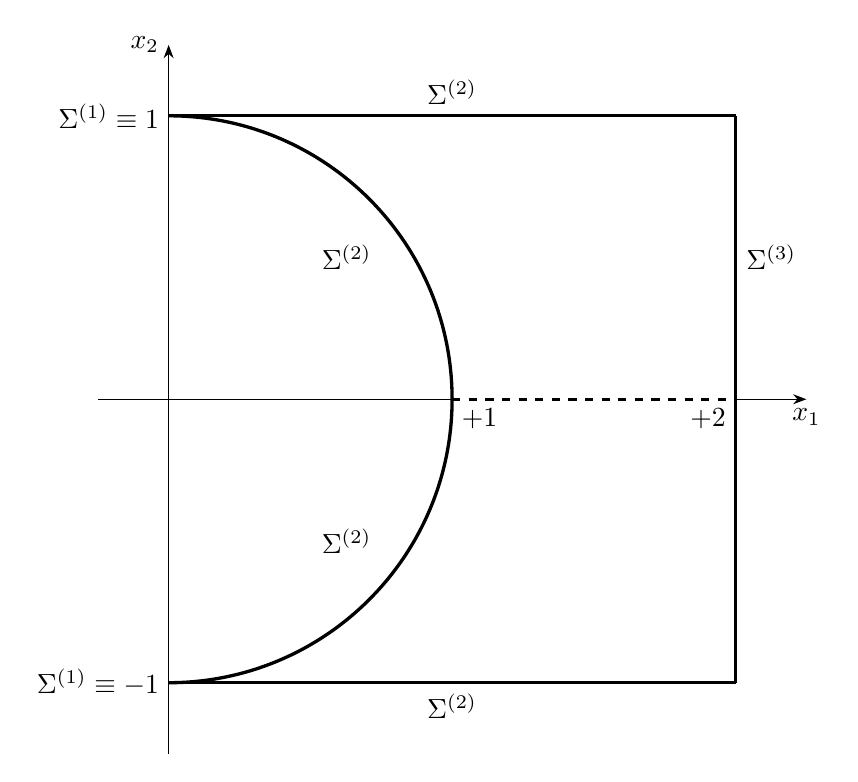
\begin{tikzpicture}[>=Stealth,scale=0.9]
		\draw (-1,0) -- (4,0);
		\draw[->] (8,0) -- (9,0) node[anchor=north] {$x_1$};
		\draw[->] (0,-5) -- (0,5) node[anchor=east] {$x_2$};
		
		\draw[very thick] (0,4) -- (4,4) node[anchor=south] {$\Sigma^{(2)}$} -- (8,4);
		\draw[very thick] (0,-4) -- (4,-4) node[anchor=north] {$\Sigma^{(2)}$} -- (8,-4);
		\draw[very thick] (8,4) -- (8,2) node[anchor=west] {$\Sigma^{(3)}$} -- (8,-4);
		
		\draw[very thick, dashed] (4,0) -- (8,0);
		
		\node[below left] at (8,0) {$+2$};
		\node[below right] at (4,0) {$+1$};
		
		\node[left] at (0,4) {$\Sigma^{(1)} \equiv 1$};
		\node[left] at (0,-4) {$\Sigma^{(1)} \equiv -1$};
		
		\node[left] at (3,2) {$\Sigma^{(2)}$};
		\node[left] at (3,-2) {$\Sigma^{(2)}$};
		
		\draw[very thick] (0,-4) arc (-90:90:4);
	\end{tikzpicture}
	\caption{}
	\label{fig:5}
\end{figure}

\begin{figure}
	\centering
	\usetikzlibrary {arrows.meta}
	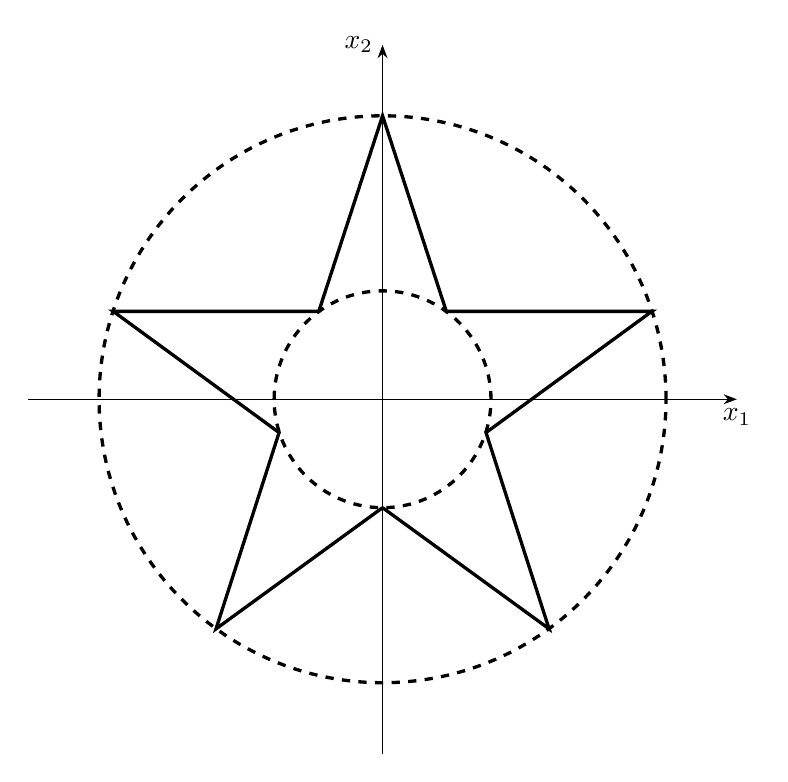
\begin{tikzpicture}[>=Stealth,scale=0.9]
		\draw[->] (-5,0) -- (5,0) node[anchor=north] {$x_1$};
		\draw[->] (0,-5) -- (0,5) node[anchor=east] {$x_2$};
		
		\draw[very thick] (0,-1.53) -- (2.35,-3.24) -- (1.46,-0.47) -- (3.80,1.24) -- (0.90,1.24) -- (0,4) -- (-0.90,1.24) -- (-3.80,1.24) -- (-1.46,-0.47) -- (-2.35,-3.24) -- (0,-1.53); 
		
		\draw[very thick, dashed] (4,0) arc (0:360:4);
		\draw[very thick, dashed] (1.53,0) arc (0:360:1.53);
	\end{tikzpicture}
	\caption{}
	\label{fig:6}
\end{figure}

As last example let us consider the mixed elliptic-parabolic equation:
\begin{equation*}
	k\left(x_{2}\right) u_{x_{1} x_{1}}+u_{x_{2} x_{2}}=f ;
\end{equation*}
$k\left(x_{2}\right)$ is a function positive for $x_{2}>0$ and vanishing for $x_{2} \leq 0$. 
Let $A$ be the domain bounded by: (1.) a regular arc $\mathcal{C}_{1}$ joining the two points $0$ and $1$ of the $x_{1}$-axis and entirely lying in the halfplane $x_{2}>0$; (2.) an arc $\mathcal{C}_{2}$ (with $x_{2}<0$) joining the origin with the point $(1,-1)$ and with a tangent nowhere parallel to the $x_{2}$-axis; (3.) the segment $\mathcal{C}_{3}$ joining $(1,0)$ and $(1,-1)$.
In this case we have $\Sigma^{(3)}=\mathcal{C}_{1} \cup \mathcal{C}_{2}$, $\Sigma^{(1)}=\mathcal{C}_{3}$. 
We can indeed prescribe $u$ on $\mathcal{C}_{1}$ and $\mathcal{C}_{2}$.

In the next sections it will be shown in what sense and under what further conditions there exist unique solutions of \eqref{eq:1.1} (in particular, solutions of the example problems) which are continuously dependent on the data.

\begin{figure}
	\centering
	\usetikzlibrary {arrows.meta}
	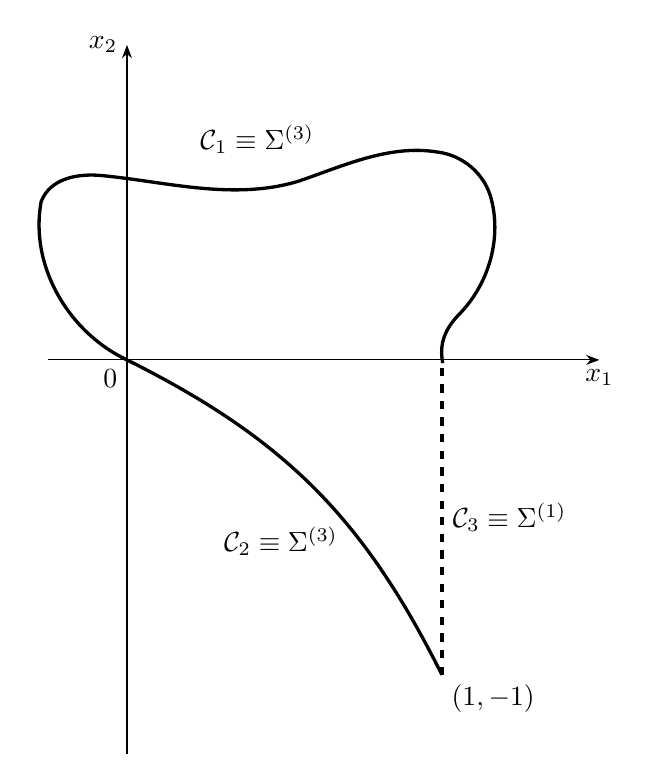
\begin{tikzpicture}[>=Stealth]
		\draw[->] (-1,0) -- (6,0) node[anchor=north] {$x_1$};
		\draw[->] (0,-5) -- (0,4) node[anchor=east] {$x_2$};
		
		\node[below left] at (0,0) {$0$};
		\node[below right] at (4,-4) {$(1,-1)$};
		
		\draw[very thick, dashed] (4,-4) -- (4,-2) node[anchor=west] {$\mathcal{C}_3\equiv\Sigma^{(1)}$} -- (4,0);
		\draw[very thick] (4,-4) .. controls (3,-2) and (2,-1) .. (0,0);
		\draw [very thick] (0,0)
		.. controls ++(-7.4mm,3.5mm) and ++(-1.5mm,-8.2mm) .. ++(-10.9mm,20.1mm)
		.. controls ++(1.2mm,3.1mm) and ++(-2.9mm,0.3mm) .. ++(7.8mm,3.3mm)
		.. controls ++(8.2mm,-0.8mm) and ++(-8.2mm,-2.5mm) .. ++(24.9mm,-0.7mm)
		.. controls ++(5.6mm,1.9mm) and ++(-6.1mm,1.0mm) .. ++(17.6mm,3.7mm)
		.. controls ++(3.3mm,-0.4mm) and ++(-0.8mm,3.3mm) .. ++(6.9mm,-6.1mm)
		.. controls ++(1.3mm,-5.2mm) and ++(3.7mm,3.7mm) .. ++(-4.2mm,-14.6mm)
		.. controls ++(-1.6mm,-1.7mm) and ++(-0.5mm,2.6mm) .. ++(-2mm,-6.1mm)
		;
		
		\node[below left] at (2.8,-2) {$\mathcal{C}_2 \equiv \Sigma^{(3)}$};
		\node[above left] at (2.5,2.5) {$\mathcal{C}_1 \equiv \Sigma^{(3)}$};
		
	\end{tikzpicture}
	\caption{}
	\label{fig:7}
\end{figure}

\section{Integral a priori estimates and maximum principles}
\label{sec:3}

Let us define as class $C_{L}$ the family of all real functions $u$ satisfying the following conditions:
\begin{enumerate}[label=\alph*.]
	\item $u$ is continuous with its first derivatives in $A \cup \Sigma$, [$u \in C^{1}(A \cup \Sigma)$],
	\item $u$ has continuous second derivatives in $A$, [$u \in C^{2}(A)$],
	\item the function $L(u)$ is bounded in $A$.
\end{enumerate}
We shall denote by $L^{*}$ the formal adjoint of the operator $L$:
\begin{equation*}
	\begin{aligned}
		L^{*}(u)&=(a^{ij})_{x_i x_{j}}-(b^i u)_{x_i}+c u \\
		&\equiv a^{i j} u_{x_{i} x_{j}}+b^{* i} u_{x_{i}}+c^{*} u,
	\end{aligned}
\end{equation*}
where
\begin{equation*}
	b^{*i} = 2 a^{ij}_{x_j} - b^i,
	\quad
	c^* = a^{ij}_{x_i x_j} - b^i_{x_i} + c.
\end{equation*}

\begin{thm}{I} \label{thm:I}
	Let $p$ be a real number such that $1 \leq p<+\infty$ and let a function $w$ exist belonging to $C^{2}(A \cup \Sigma)$ and satisfying the condition
	\begin{equation}
		\label{eq:3.1}
		w \leq 0, \quad 
		L^{*}(w)+(p-1) c w>0 \text{ in } A \cup \Sigma.
	\end{equation}
	For any function $u$ of $C_{L}$ vanishing almost everywhere on $\Sigma^{(2)} \cup \Sigma^{(3)}$, the following inequality holds:
	\begin{equation}
		\label{eq:3.2}
		\boxed{
		\left(\int_{A}|u|^{p} \dd x\right)^{\frac{1}{p}} \leq p \frac{\max_{A \cup \Sigma}|w|}{\min_{A\cup\Sigma} \left[L^{*}(w)+(p-1) c w\right]}\left(\int_{A}|L(u)|^{p} \dd x\right)^{\frac{1}{p}}.}
	\end{equation}
\end{thm}

\begin{proof}
	Let $\delta$ denote an arbitrary positive number. 
	By using Green's integral theorem the following identity is shown:
	\begin{equation}
		\label{eq:3.3}
		\begin{split}
			\int_A & \{ 
			(u^2+\delta)^{\frac p 2} L^*(w) - w \big( p[(p-1)u^2+\delta] (u^2+\delta)^{\frac p 2 - 2} a^{hk} u_{x_h} u_{x_k} \\
			& + p(u^2+\delta)^{\frac p 2 -1} u L(u) + c (u^2+\delta)^{\frac p 2 - 1} [(1-p)u^2+\delta] \big) \} \dd x \\
			& = \int_{\Sigma^{(1)}\cup\Sigma^{(2)}} w(u^2+\delta)^{\frac p 2} b \dd \sigma + \int_{\Sigma^{(3)}} [p^2(u^2+\delta)^{\frac p 2 - 1} w u a^{hk}u_{x_h} n_k \\
			& \quad - (u^2+\delta)^{\frac p 2}(a^{hk}w_{x_h}n_k-bw)] \dd \sigma.			
		\end{split}
	\end{equation}
	Since a.e.\ on $\Sigma^{(1)}$, $b\geq0$; and $a^{hk}u_{x_h}u_{x_k} \geq 0$, $w \leq 0$ in $A\cup\Sigma$, by the assumed hypotheses on $u$, it follows:
	\begin{equation*}
		\begin{aligned}
			&\int_{A}\left(u^{2}+\delta\right)^{\frac{p}{2}}\left\{L^{*}(w)-c w\left(u^{2}+\delta\right)^{-1}\left[(1-p) u^{2}+\delta\right]\right\} \dd x \\
			&\leq p \int_{A}\left(u^{2}+\delta\right)^{\frac{p}{2}-1} u w L(u) \dd x+\delta^{\frac{p}{2}}\left[\int_{\Sigma^{(2)}} w b \dd \sigma-\int_{\Sigma^{(3)}}\left(a^{h k} w_{x_{h}} n_{k}-b w\right) \dd \sigma\right].
		\end{aligned}
	\end{equation*}
	We observe that 
	\begin{gather*}
		\lim_{\delta \rightarrow 0}\left(u^{2}+\delta\right)^{\frac{p}{2}}\left\{L^{*}(w)-c w\frac{(1-p) u^{2}+\delta}{u^{2}+\delta}\right\}=\left(u^{2}\right)^{\frac{p}{2}}\left\{L^{*}(w)-(1-p) c w\right\},
		\\
		\lim _{\delta \rightarrow 0}\left(u^{2}+\delta\right)^{\frac{p}{2}-1} u=\left(u^{2}\right)^{\frac{p}{2}-1} u,
	\end{gather*}
	uniformly with respect to $x$ in $A \cup \Sigma$.

	From \eqref{eq:3.3} it follows
	\begin{equation}
		\label{eq:3.4}
		\int_{A}|u|^{p} \dd x \leq p \frac{\max_{A\cup\Sigma} |w|}{\min_{A\cup\Sigma} \left[L^{*}(w)+(p-1) c w\right]} \int_{A}|u|^{p-1}|L(u)| \dd x
	\end{equation}
	This coincides with \eqref{eq:3.2} for $p=1$. 
	For $p>1$, \eqref{eq:3.2} follows from \eqref{eq:3.4} by applying the Schwarz-Hölder inequality to the integral on the right hand side.
\end{proof}

\begin{thm}{II}
	If $c < 0$ in $A\cup\Sigma$, or $c^* < 0$ in $A\cup \Sigma$, $p$ and $w$ exist satisfying \eqref{eq:3.1}.
\end{thm}

\begin{proof}
	In the first case ($c<0$) we can assume $w\equiv-1$ and $p$ large enough, that 
	\begin{equation*} \min_{A\cup\Sigma} \left[-a_{x_{h} x_{k}}^{h k}+b_{x_{h}}^{h}-p c\right]>0 \quad \text{in } A\cup\Sigma.
	\end{equation*}
	In the second case ($c^{*}<0$) we assume $w \equiv-1$ and $p$ so small that
	$$	\min_{A\cup\Sigma} \left[(1-p) c-c^{*}\right]>0$$ (in particular $p=1$).
\end{proof}

It is obvious that
\begin{thm}{III} \label{thm:III}
	If $c<0$ and $c^{*}<0$ in $A \cup \Sigma$, then for any $p \geq 1$ the condition \eqref{eq:3.1} is satisfied by assuming $w \equiv-1$.
\end{thm}

\begin{thm}{IV} \label{thm:IV}
	Let $c$ be negative in $A \cup \Sigma$. 
	Let $w$ denote an arbitrary function of $C^{2}\left(A \cup \Sigma\right)$ negative in $A \cup \Sigma$ and $p_0$ a real number such that $L^*(w)+\left(p_{0}-1\right)cw\geq 0$ in $A \cup \Sigma$. For any $p$ such that $p>p_{0}$, $p\geq 1$, and for any $u \in C_L$, vanishing a.e.\ on 
	$\Sigma^{(2)} \cup \Sigma^{(3)}$, the following inequality holds:
	\begin{equation}
		\label{eq:3.5}
		\boxed{
		\left(\int_{A}|u| c w \dd x\right)^{\frac{1}{p}} \leq \frac{p}{p-p_{0}}\left(\int_{A}\left|\frac{L(u)}{c}\right|^{p} cw \dd x\right)^{\frac{1}{p}}.
		}
	\end{equation}
\end{thm}

\begin{proof}
	Since $w$ satisfies for $p>p_{0}$ the conditions \eqref{eq:3.1}, from \eqref{eq:3.3} for $p>p_{0}$, $p \geq 1$, it follows (for $\delta \to 0$) that
	\begin{equation*}
		\int_{A}\left(u^{2}\right)^{\frac{p}{2}}\left[L^{*}(w)-(1-p) c w\right] \dd x \leq p \int_{A}\left(u^{2}\right)^{\frac{p}{2}-1} u w L(u) \dd x.
	\end{equation*}
	Since $L^{*}(w)-(1-p) c w \geq\left(p-p_{0}\right) w$, from the previous inequality it follows that
	\begin{equation}
		\label{eq:3.6}
		\int_{A}|u|^{p} c w \dd x \leq \frac{p}{p-p_{0}} \int_{A}|u|^{p-1}|w||L(u)| \dd x
	\end{equation}
	which coincides with \eqref{eq:3.5} for $p=1$. 
	In the case $p>1$ we have
	\begin{equation}
		\label{eq:3.7}
		\begin{split}
			\int_{A} & |u|^{p-1}|L(u)||w| \dd x \\
			& \leq \left(\int_{A}\left[|u|^{p-1}|c|^{\frac{p-1}{p}}\right]^{\frac{p}{p-1}}|w|\dd x\right)^{\frac{p-1}{p}}  \left(\int_{A}\left[|L(u)||c|^{\frac{1-p}{p}}\right]^{p}|w| \dd x\right)^{\frac{1}{p}} \\
			& = \left(\int_{A}|u|^{p}|c||w| \dd x\right)^{\frac{p-1}{p}}\left(\int_{A}\left|\frac{L(u)}{c}\right|^{p}|c||w| \dd x\right)^{\frac{1}{p}} \\
			& =\left(\int_{A}|u|^{p} c w \dd x\right)^{\frac{p-1}{p}}\left(\int_{A}\left|\frac{L(u)}{c}\right|^{p} c w \dd x\right)^{\frac{1}{p}}
		\end{split}
	\end{equation}
	From \eqref{eq:3.6} and \eqref{eq:3.7}, the inequality \eqref{eq:3.5} follows.
\end{proof}

From \eqref{eq:3.5} we deduce the following maximum principle:

\begin{thm}{V} \label{thm:V}
	Let $c$ be negative in $A \cup \Sigma$. 
	For any $u \in C_{L}$ vanishing almost everywhere on $\Sigma^{(2)} \cup \Sigma^{(3)}$ the inequality holds (\ref{note:3}):
	\begin{equation}
		\label{eq:3.8}
		\boxed{\max_{A\cup\Sigma} |u| \leq \underset{A}{\operatorname{l.u.b.}} \left|\frac{L(u)}{c}\right|}
	\end{equation}
\end{thm} 

\begin{proof}
	This follows from \eqref{eq:3.5} for $p \rightarrow+\infty$.
\end{proof}

\begin{thm}{VI} \label{thm:VI}
	When hypotheses of theorems \ref{thm:III} or \ref{thm:V} are satisfied, a uniqueness theorem holds for the problem \eqref{eq:1.1} with ${\Sigma}_N=\varnothing$ in the class
	$C_{L}$.
\end{thm}

It is evident that for particular classes of elliptic-operators $L$ (as an instance first order operators) theorems \ref{thm:I} - \ref{thm:VI} remain valid with the same proof, assuming $C_{L}$ to be defined in a more general way (not 	necessarily requiring the existence and the continuity of all the derivatives of $u$ in $A$.)

We want now to consider some estimates in connection with problem \eqref{eq:1.1} in the general case (i.e., $\Sigma_N$ not empty).

\begin{thm}{VII} \label{thm:VII}
	Let $p$ be a real number: $1 \leq p<+\infty$ and $w$ a function of $C^{2}(A \cup \Sigma)$ such that:
	\begin{gather}
		\tag{3.1}
		w \leq 0, \quad L^{*}(w)+(p-1) c w>0
		\quad \text{on } A \cup \Sigma \\
		\nonumber
		a^{h k} w_{x_{h}}n_{k}-b w \geq 0 \quad \text{a.e.\ on } \Sigma^{(3)}-\overline{\Sigma^{(3)}_D}. \quad (\ref{note:4})
	\end{gather}
	For any $u \in C_{L}$ satisfying a.e.\ the conditions
	\begin{equation*}
		u = 0 \text{ on } \Sigma^{(2)} \cup \overline{\Sigma^{(3)}_D}, \quad 
		a^{hk} u_{x_h} n_k = 0 \text{ on } \Sigma^{(3)}-\overline{\Sigma^{(3)}_D}
	\end{equation*}
	the inequality \eqref{eq:3.2} holds.
\end{thm}

The proof is analogous to the proof of theorem \ref{thm:I} (\ref{note:5}).

\begin{thm}{VIII} \label{thm:VIII}
	Let $c$ be negative in $A \cup \Sigma$ and a negative function $w$ in $A\cup\Sigma$ exist such that $a^{hk} w_{x_h}n_k-bw\geq 0$ on $\Sigma_N^{(3)}$. 
	Then $p\geq 1$ exists such that \eqref{eq:3.1} is satisfied.
\end{thm}

The proof is obvious.

\begin{thm}{IX} \label{thm:IX}
	For the same hypotheses of the previous theorem, let $p_{0}$ be a real number such that $L^{*}(w)+\left(p_{0}-1\right) c w \geq 0$.
	For $p>p_{0}$, $p \geq 1$ and any $u$ satisfying the conditions of theorem \ref{thm:VII}, the inequality \eqref{eq:3.5} holds.
\end{thm}

This theorem is proved as theorem \ref{thm:IV}.

\begin{thm}{X}
	For the same hypotheses of theorem \ref{thm:VIII}, the Inequality \eqref{eq:3.8} holds for any $u$ satisfying the conditions of theorem \ref{thm:VII}.
\end{thm}

From theorems \ref{thm:VII} and \ref{thm:IX} uniqueness theorems follow for the problem \eqref{eq:1.1} in the class $C_{L}$.

\begin{thm}{XI} \label{thm:XI}
	For a fixed $p$ ($1 \leq p<+\infty$) let a function $w \in C^{2}(A \cup \Sigma)$ exist satisfying the following conditions:
	\begin{equation*}
		\begin{aligned}
			&w \leq 0, \quad L^{*}(w)+(p-1) c w>0 \quad \text{in } A \cup \Sigma, \\
			&w=0 \text{ a.e.\ on } \ovdir,\quad a^{h k} w_{x_{h}} n_{k}-b w \geq 0 \text{ a.e.\ on } \Sigma^{(3)}-\ovdir .
		\end{aligned}
	\end{equation*}
	For any $u\in C_L$, such that: $L(u)=0$ in $A$, $a^{h k} u_{x_{h}}n_{k}=0$ a.e.\ on $\overline{\Sigma^{(3)}}-\overline{\Sigma_D^{(3)}}$, the inequality holds
	\begin{equation}
		\label{eq:3.9}
		\boxed{
		\begin{aligned}
			\left(\int_A |u|^p \dd x\right)^{\frac 1 p}
			& \leq 
			\left\{\frac{\underset{\Sigma^{(2)}}{\operatorname{l.u.b.}}|bw|}{\underset{A\cup\Sigma}{\min} [L^*(w)+(p-1)cw]}\right\}^{\frac 1 p} \left(\int_{\Sigma^{(2)}} |u|^p \dd\sigma \right)^{\frac 1p} \\
			& + \left\{\frac{\underset{\overline{\Sigma^{(3)}_D}}{\operatorname{l.u.b.}}|a^{hk}w_{x_h}n_k|}{\underset{A\cup\Sigma}{\min} [L^*(w)+(p-1)cw]}\right\}^{\frac 1 p} \left(\int_{\overline{\Sigma^{(3)}_D}} |u|^p \dd\sigma \right)^{\frac 1p}.
		\end{aligned}}
	\end{equation}
\end{thm}

\begin{proof}
	From \eqref{eq:3.3} and the hypotheses for $u$ and $w$, it follows that
	\begin{equation*}
		\begin{aligned}
			&\int_{A}\left\{\left(u^{2}+\delta\right)^{\frac{p}{2}} L^{*}(w)-c w\left(u^{2}+\delta\right)^{\frac{p}{2}-1}\left[(1-p) u^{2}+\delta\right]\right\} \dd x \\
			&\leq \int_{\Sigma^{(2)}} b w\left(u^{2}+\delta\right)^{\frac{p}{2}} \dd \sigma-\int_{\ovdir}\left(u^{2}+\delta\right)^{\frac{p}{2}} a^{h k} w_{x_{h}} n_{k} \dd \sigma.
		\end{aligned}
	\end{equation*}
	For $\delta \rightarrow 0$
	\begin{equation*}
		\int_{A}\left(u^{2}\right)^{\frac{p}{2}}\left[L^{*}(w)+(p-1) c w\right] \dd x \leq \int_{\Sigma^{(2)}} w\left(u^{2}\right)^{\frac{p}{2}} b \dd \sigma-\int_{\ovdir}\left(u^{2}\right)^{\frac{p}{2}} a^{h k} w_{x_h} n_{k} \dd \sigma ;
	\end{equation*}
	\eqref{eq:3.9} follows easily from this inequality.
\end{proof}

\begin{thm}{XII}
	Let $c$ be negative in $A \cup \Sigma$ and a function $w \in C^{2}(A \cup \Sigma)$ exist satisfying the conditions:
	\begin{equation*}
		w<0 \text{ in } A \cup \Sigma, \quad 
		a^{h k} w_{x_{h}} n_{k}-b w \geq 0 \text{ on } \Sigma^{(3)}-\ovdir.
	\end{equation*}
	For any $u \in C_{L}$ satisfying the conditions of theorem \ref{thm:XI} the following maximum principle holds:
	\begin{equation}
		\label{eq:3.10}
		\boxed{
		\max_{A\cup\Sigma} |u|=\max_{\overline{\Sigma^{(2)}} \cup \ovdir} |u|.}
	\end{equation}
\end{thm}

\begin{proof}
	If $p$ is an arbitrary even integer, we can use \eqref{eq:3.3} with $\delta=0$.
	Under the assumed hypotheses for $w$ and $u$ we then obtain
	\begin{equation}
		\label{eq:3.11}
		\begin{split}
			\min_{A\cup\Sigma} & [L^*(w) + (p-1)cw] \int_A u^p \dd x \leq \underset{\Sigma^{(2)}}{\operatorname{l.u.b.}} |bw| \int_{\Sigma^{(2)}} u^p \dd \sigma \\
			& + p \max_{\overline{\Sigma^{(3)}_D}} \int_{\overline{\Sigma^{(3)}_D}} |u|^{p-1} |a^{hk} u_{x_h} n_k| \dd \sigma
			+ \underset{\overline{\Sigma^{(3)}_D}}{\operatorname{l.u.b.}} |a^{hk} w_{x_h} n_k - bw| \int_{\overline{\Sigma^{(3)}_D}} u^p \dd \sigma.
		\end{split}
	\end{equation}

	Let us first suppose $u=0$ a.e.\ on $\ovdir$. 
	Since two positive numbers $P_{1}$ and $P_{2}$ exist such that for $p$ large enough, $P_{1} \leq \min_{A\cup\Sigma} \left[L^{*}(w)+(p-1) c w\right] \leq P_{2} p$, it follows that $\lim_{p \rightarrow \infty}\left\{\min _{A \cup \Sigma}\left[L^{*}(w)+(p-1) c w\right]\right\}^{\frac{1}{p}}=1$.
	From \eqref{eq:3.11} the inequality
	\eqref{eq:3.10} follows easily.
	
	Let us now consider the case that $u$ does not vanish a.e.\ on $\ovdir$.
	By considering the Schwarz-Hölder inequality,
	\begin{equation*}
		\int_{\ovdir} |u|^{p-1} |a^{hk} u_{x_h} n_k| \dd \sigma 
		\leq \left(\int_{\ovdir} u^p \dd \sigma\right)^{\frac{p-1}{p}} \left(\int_{\ovdir} |a^{hk}u_{x_h} n_k|^p \dd \sigma\right)^{\frac 1 p},
	\end{equation*}
	from \eqref{eq:3.11} we get
	\begin{equation}
		\label{eq:3.12}
		\min_{A \cup \Sigma}\left[L^{*}(w)+(p-1) c w\right] \int_{A} u^{p} \dd \sigma \leq K_{p} \int_{\Sigma^{(2)} \cup \ovdir} u^{p} \dd \sigma
	\end{equation}
	where
	\begin{equation*}
		\begin{split}
			K_p = \lub{\Sigma^{(2)}} |bw| & + p \max_{\ovdir} |w| \left(\int_{\ovdir} u^p \dd \sigma\right)^{-\frac 1p} \left(\int_{\ovdir} |a^{hk} u_{x_h} n_k|^p \dd \sigma \right)^{\frac 1p}  \\
			& 			+ \lub{} |a^{hk} w_{x_h} n_k-bw|.
		\end{split}
	\end{equation*}

	Let $M$ be a positive number such that, for any even integer $p$,
	\begin{equation*}
		\left(\int_{\ovdir} u^p \dd \sigma \right)^{-\frac 1p} \left(\int_{\ovdir} |a^{hk}u_{x_h}n_k|^p \right)^{\frac 1p} \leq M.
	\end{equation*}
	We get
	\begin{equation*}
		\begin{split}
			K_p^{\frac1p}
			& \leq \left[ \lub{\Sigma^{(2)}} |bw| + p \max_{\ovdir} |w|M + \lub{\ovdir} |a^{hk}w_{x_h}n_k-bw|\right]^{\frac 1p}
			\\
			& \leq p^{\frac 1p}\left[ \lub{\Sigma^{(2)}} |bw| + M \max_{\ovdir} |w| + \lub{\ovdir} |a^{hk}w_{x_h}n_k-bw|\right]^{\frac 1p}
		\end{split}
	\end{equation*}
	and
	\begin{equation*}
		\underset{p\to+\infty}{\operatorname{max~lim}} K_p^{\frac 1p} \leq 1.
	\end{equation*}

	Let $p_0$ be such that $\min_{A\cup\Sigma} [L^*(w)+(p-1)cw] \geq 0$ for $p > p_0$.
	For $p > p_0$, from \eqref{eq:3.12} we obtain
	\begin{equation*}
		\left(\min_{A\cup\Sigma}[L^*(w)+(p-1)cw]\right)^{\frac1p}
		\left(\int_A u^p \dd \sigma\right)^{\frac1p}
		\leq
		K_p^{\frac 1p}
		\left(\int_{\Sigma^{(2)}\cup\ovdir} u^p \dd\sigma\right)^{\frac1p}
	\end{equation*}
	and for $p \to \infty$ we obtain \eqref{eq:3.10}.
\end{proof}

\begin{thm}{XIII} \label{thm:XIII}
	Let $c$ be negative in $A\cup\Sigma$. 
	For any solution $u$ of $L(u)$ of the class $C_L$ not identically vanishing in $A$, the following maximum principle holds:
	\begin{equation*}
		\boxed{
			\max_A |u| < \max_{\overline{\Sigma^{(2)}} \cup \overline{\Sigma^{(3)}}} |u|.
		}
	\end{equation*}
\end{thm}

\begin{proof}
	Let us assume $\Sigma_{D}^{(3)}=\Sigma^{(3)}$. Then as a function $w$ satisfying the hypotheses of the previous theorem we can select $w \equiv-1$. 
	In this case the inequality \eqref{eq:3.10} is the following:
	\begin{equation*}
		\max_{A \cup \Sigma}|u|=\max_{\overline{\Sigma^{(2)}} \cup \overline{\Sigma^{(3)}}} |u|.
	\end{equation*}
	Since $\max_{A \cup \Sigma}|u| = \max _{A \cup \Sigma} u$ or $\max_{A \cup \Sigma}|u| = - \min_{A \cup \Sigma} u$, it follows that $u$ has in $A\cup\Sigma$ a positive maximum or a negative minimum.
	
	From the condition $c<0$, by a well known argument, it follows that such a positive maximum or negative minimum cannot be attained in a point of $A$ (\ref{note:6}). 
	Therefore
	\begin{equation*}
		|u(x)| < \max_{A\cup\Sigma} |u|
		\quad \text{for } x \in A.
	\end{equation*}
	
	It is evident that the same argument could be given to establish the maximum principle (as in theorem \ref{thm:XIII}) in the general case $\Sigma_{N}^{(3)} \neq \varnothing$.
\end{proof}


\section{An abstract existence principle}

In order to establish the necessary and sufficient condition for the existence of a weak solution of the problem \eqref{eq:1.1}, we shall make use of an abstract existence principle in Banach spaces.

Let $\mathscr{V}$ be an abstract manifold linear with respect to the real field and $B_{1}$ and $B_{2}$ real Banach spaces. Let $M_{i}$ ($i=1,2)$ be a linear homomorphism of $\mathscr{V}$ into ${B}_{i}$; $\phi$ and $\psi$ denote vectors of the adjoint spaces $B_{1}^{*}$ and $B_{2}^{*}$, respectively. We consider for any ${v} \in \mathscr{V}$ the following functional equation:
\begin{equation} \label{eq:4.1}
	\left\langle\phi, {M}_{1}(v)\right\rangle=\left\langle\psi, M_{2}(v)\right\rangle,
\end{equation}
where $\phi$ is a given vector and $\psi$ is the unknown. Let $\mathscr{V}_2$ be the kernel of the homomorphism $M_{2}$. The given vector $\phi$ must satisfy the following necessary conditions:
\begin{equation} \label{eq:4.2}
	\left\langle\phi, M_{1}\left(v_{2}\right)\right\rangle=0
	\text{ for any } 
	v_{2} \in \mathscr{V}_{2} .
\end{equation}
Let $M_{1}\left(\mathscr{V}_{2}\right)$ denote the image of $\mathscr{V}_{2}$ on $B_{1}$, for $M_{1}$ and $\overline{M_{1}\left(\mathscr{V}_{2}\right)}$ its closure. Let us consider the Banach factor-space: $Q={B}_{1} / \overline{M_{1}\left(\mathscr{V}_{2}\right)}$.
Let $\mathscr{M}_{1}$ be the homomorphism that maps $v \in \mathscr{V}$ in the equivalence class $\left[M_{1}(v)\right]$ of $Q$.

The following existence principle holds:

\begin{thm}{XIV} \label{XIV}
	A solution $\psi$ of the functional equation \eqref{eq:4.1} exists for any fixed $\phi$ satisfying~\eqref{eq:4.2}, when and only when a constant $K$ exists such that for any $v \in \mathscr{V}$ the inequality holds
	\begin{equation} \label{eq:4.3}
		\left\|\mathscr{M}_{1}(v)\right\|_{Q} \leq K\left\|M_{2}(v)\right\|_{B_{2}}.
	\end{equation}
\end{thm}

Let $\mathscr{A}$ be the (closed) subspace of $B_{2}^*$, consisting of the vectors $\psi$, solutions of the ``homogeneous'' problem,
\begin{equation*}
	\left\langle\psi, M_{2}(v)\right\rangle=0 \text{, for any } v \in \mathscr{V}.
\end{equation*}
We denote by $\mathscr{F}$ the Banach factor-space: $\mathscr{F}=B_{2}^* / \mathscr{A}$. For any $\phi \in B_{1}^*$ satisfying the compatibility condition \eqref{eq:4.2} (that is to say for any element of the adjoint space $Q^*$) an element $\Psi$ of $\mathscr{F}$ is uniquely determined such that if $\psi$ is any element in the equivalence class $\Psi$, then $\psi$ is a solution of \eqref{eq:4.1}.

\begin{thm}{XV} \label{XV}
	The element $\Psi$ of $\mathscr{F}$ corresponding to $\phi \in B_{1}^{*}$ satisfying the compatibility conditions \eqref{eq:4.2} satisfies the inequality
	\begin{equation} \label{eq:4.4}
		\|\Psi\|_{\mathscr{F}} \leq K\left\|{\phi}\right\|_{B_{1}^{*}}.
	\end{equation}
\end{thm}
Inequality \eqref{eq:4.4} is said to be the dual inequality of \eqref{eq:4.3}.

\section{Existence of weak solutions for problem \texorpdfstring{\eqref{eq:1.1}}{(1.1)}}

Let $u \in C_{L}$ and $v \in C_{L^*}$. Then the Green's identity holds
\begin{equation}
	\label{eq:5.1}
	\int_{A}(v L(u)-u L^*(v)) \dd x
	=\int_{\Sigma^{(3)}} \left[u a^{h k} v_{x_{h}} n_{k}-v a^{h k} u_{x_{h}}n_k \right] \dd \sigma
	- \int_{\Sigma^{(1)}\cup\Sigma^{(2)}} u v b \dd \sigma.
\end{equation}

Let us suppose that $u$ satisfies the boundary conditions
\begin{equation}
	\label{eq:5.2}
	u = 0 \text{ a.e.\ on } \Sigma^{(2)} \cup \Sigma^{(3)}_D,
	\quad 
	a^{hk} u_{x_h} n_k = 0 \text{ a.e.\ on } \Sigma^{(3)}_N.
\end{equation}

From \eqref{eq:5.1} it follows easily that
\begin{equation*}
	\begin{split}
		\int_{A} (u L^*(v)-v L(u)) \dd x
		=
		\int_{\Sigma^{(1)}} u v b \dd \sigma
		& + 
		\int_{\overline{\Sigma^{(3)}_D}} v a^{h k} u_{x_{h}} n_{k} \dd \sigma \\
		& -
		\int_{\Sigma^{(3)} \setminus \overline{\Sigma^{(3)}_D}} u (a^{h k} v_{x_{h}} n_{k}-bv) \dd \sigma.
	\end{split}
\end{equation*}

Let $\mathscr{V}$ be the linear manifold of the functions of $C_{L^*}$ such that for any $u \in C_{L}$ satisfying \eqref{eq:5.2}
\begin{equation*}
		\int_{\Sigma^{(1)}} u v b \dd \sigma
	+ 
	\int_{\overline{\Sigma^{(3)}_D}} v a^{h k} u_{x_{h}} n_{k} \dd \sigma
	-
	\int_{\Sigma^{(3)} \setminus \overline{\Sigma^{(3)}_D}} u (a^{h k} v_{x_{h}} n_{k}-bv) \dd \sigma
	= 0.
\end{equation*}
Let us set: $L(u)=f$. It follows that
\begin{equation}
	\label{eq:5.3}
	\int_{A} v f \dd x=\int_{A} u L^{*}(v) \dd x
\end{equation}
for any $v \in \mathscr{V}$.

We shall say that the problem \eqref{eq:1.1} [with homogeneous boundary conditions ($g\equiv0, h\equiv0$)] admits an $\mathscr{L}^{(p)}$-weak solution if for every $f \in \mathscr{L}^{(p)}(A)$ ($p > 1$), a function $u \in \mathscr{L}^{(p)}(A)$ exists satisfying \eqref{eq:5.3} for any $v \in \mathscr{V}$.


From theorems \ref{XIV}, \ref{XV} and by the representation theorems of linear bounded functionals in the $\mathscr{L}^{(p)}$-spaces this general condition follows:

\begin{thm}{XVI}
	An $\mathscr{L}^{(p)}$-weak solution of problem \eqref{eq:1.1} exists for any
	$f \in \mathscr{L}^{(p)}(A)$ such that
	\begin{equation*}
		\int_{A} v_{0} f \dd x=0 \quad
		\left(v_{0} \in \mathscr{V}, L^{*}\left(v_{0}\right)=0\right)
	\end{equation*}
	when and only when a constant $K$ exists such that:
	\begin{equation}
		\label{eq:5.4}
		\underset{v_0 \in \mathscr{V}_0}{\operatorname{g.l.b.}}
		\left(\int_{A} |v+v_{0}|^{\frac{p}{p-1}} \dd x\right)^{\frac{p-1}{p}} \leq K\left(\int_{A}\left|L^{*}(v)\right|^{\frac{p}{p-1}} \dd x\right)^{\frac{p-1}{p}}
	\end{equation}
	where $\mathscr{V}_{0}$ is the subset of $\mathscr{V}$ of all the functions which are solutions of the adjoint equation $L^{*}(v)=0$.
	
	When \eqref{eq:5.4} holds, any $\mathscr{L}^{(p)}$-weak solution satisfies the inequality,
	\begin{equation}
		\label{eq:5.5}
		\underset{u_0 \in \mathscr{U}_0}{\operatorname{g.l.b.}}
		\left(\int_{A} |u+u_{0}|^p \dd x\right)^{\frac{1}{p}} \leq K\left(\int_{A}|f|^{p} \dd x\right)^{\frac{1}{p}}
	\end{equation}
	where $\mathscr{U}_{0}$ is the class of the $\mathscr{L}^{(p)}$-functions satisfying the conditions,
	\begin{equation*}
		\int_{A} u_{0} L^{*}(v) \dd x=0
	\end{equation*}
	for any $v \in \mathscr{V}$.
\end{thm}

Inequality \eqref{eq:5.5} shows that the solution $u$ of problem \eqref{eq:1.1} depends continuously -- in the $\mathscr{L}^{(p)}$ norm -- on the datum $f$, modulo the eigensolutions of the problem.

Therefore, when \eqref{eq:5.4} has been proved, it seems reasonable from the last observation to consider problem \eqref{eq:1.1} as a well posed boundary value problem.

The a priori estimates proved in \cref{sec:3} combined with theorem \ref{XV} permit us to state that,

\begin{thm}{XVII}
	Inequality \eqref{eq:5.4} holds when the hypotheses of theorem \ref{thm:VII} are satisfied.
\end{thm}

The inequality \eqref{eq:5.4} is deduced from the dual inequality of \eqref{eq:3.2}.

Other conditions for the validity of \eqref{eq:5.4} can be obtained when it is possible to apply to the functions of $\mathscr{V}$ the results of \cref{sec:3} considered with respect to the operator $L^{*}$. For simplicity let us consider the particular case $\Sigma^{(3)} \equiv \Sigma_{D}^{(3)}$ and suppose that $\mathscr{V}$ coincides with the class of functions of $C_{L^{*}}$ satisfying a.e.\ the boundary condition $v=0$ on $\Sigma^{*(2)} \cup \Sigma^{(3)}$, where $\Sigma^{*(i)}$ ($i=1,2$) is defined with respect to $L^{*}$ as $\Sigma^{(i)}$ was defined with respect to $L$.

This hypothesis on $\mathscr{V}$ will be denoted as hypothesis a). We denote by $\Sigma_{0}^{(1)}$ the subset of $\Sigma^{(1)}$ where $b=0$. The hypothesis a) is satisfied when the space spanned by the function $\eta$ defined by
\begin{equation*}
	\eta =
	\begin{cases}
		u & \text{on } \Sigma^{(1)}\cup\Sigma_0^{(1)} \\
		a^{h k} u_{x_{h}}{n}_{k} & \text{on } \Sigma^{(3)}
	\end{cases}
\end{equation*}
(for any $u \in C_{L}$ and satisfying \eqref{eq:5.2}) is dense in $\mathscr{L}^{(1)} \left(\left[\Sigma^{(1)}-\Sigma_{0}^{(1)}\right] \cup \Sigma^{(3)}\right)$.

From theorem \ref{thm:I} we deduce that

\begin{thm}{XVIII} \label{XVIII}
	If hypothesis a) is satisfied and a function $w$ exists satisfying the conditions
	\begin{equation*}
		w \leq 0, \quad 
		L(w)+\frac{1}{p-1} c^{*} w>0 \quad 
		\text{in }
		A \cup \Sigma \quad (p>1)
	\end{equation*}
	then for any $v \in \mathscr{V}$ the inequality holds
	\begin{equation*}
		\left(\int_{A}|v|^{\frac{p}{p-1}} \dd x\right)^{\frac{p-1}{p}} \leq K\left(\int_{A}\left|L^{*} w\right|^{\frac{p}{p-1}} \dd x\right)^{\frac{p-1}{p}}
	\end{equation*}
	where
	\begin{equation*}
		K=\frac{p}{p-1} \frac{\underset{A \cup \Sigma}{\max} |u|}{\underset{A \cup \Sigma}{\max} \left[L(w)+\frac{1}{p-1} c^{*} w\right]}.
	\end{equation*}
	In this case the $\mathscr{L}^{(p)}$-weak solution of problem \eqref{eq:1.1} exists for any fixed $f \in \mathscr{L}^{(p)}(A)$.
\end{thm}


Let us now suppose that a sequence of functions $u_{n}$ exist, satisfying \eqref{eq:5.2} and belonging to $C_{L}$, such that
\begin{equation}
	\label{eq:5.6}
	\lim _{n \rightarrow \infty} \int_{A}\left|u-u_{n}\right|^{p} \dd x=\lim _{n \rightarrow \infty} \int_{A}|L(u_n)-f|^{p} \dd x=0
\end{equation}
Then $u$ is said to be (according to Friedrichs) an $\mathscr{L}^{(p)}$-strong solution of problem \eqref{eq:1.1} (with homogeneous boundary condition). It is obvious that any $\mathscr{L}^{(p)}$-strong solution is a $\mathscr{L}^{(p)}$-weak solution.

We shall denote as problem \eqref{eq:1.1*} the following one $(\Sigma^{(3)}=\Sigma_{D}^{(3)})$:
\begin{equation}
	\label{eq:1.1*}
	\tag{$1.1^*$}
	L^*(v) = f \text{ in } A,
	\quad 
	v = 0 \text{ on } \Sigma^{*(2)} \cup \Sigma^{*(3)}.
\end{equation}

\begin{thm}{XIX} \label{XIX}
	Let the hypothesis a) hold. If the $\mathscr{L}^{(p)}$-weak solution ($p>1$) solution of \eqref{eq:5.3} is an $\mathscr{L}^{(p)}$-strong solution.
\end{thm}

For the existence and uniqueness of the $\mathscr{L}^{(p)}$-weak solution of \eqref{eq:5.3} it follows that the inequality holds
\begin{equation}
	\label{eq:5.7}
	\int_{A}|u|^{p} \dd x \leq K \int_{A}|f|^{p} \dd x
\end{equation}
Since only the zero function of $\mathscr{L}^{\left(\frac{p}{p-1}\right)}(A)$ is orthogonal to every $L(u)$ ($u \in C_{L}$ and satisfying \eqref{eq:5.2}) a sequence $u_{n}$ of such functions can be chosen in such a way that $L\left(u_{n}\right)$ converge to $f$; \eqref{eq:5.6} then follows from \eqref{eq:5.7}.

\section{The \texorpdfstring{$\mathscr{H}$}{H}-weak solutions}

We want now to consider a different approach to problem \eqref{eq:1.1} that appears as a natural extension to our elliptic-parabolic problems of the well known method for elliptic equations founded on energy integral. We shall only consider, for the sake of simplicity, the case $\Sigma^{(3)} \equiv \Sigma_{D}^{(3)}$ with homogeneous boundary conditions
\begin{equation} \label{eq:1.1_0}
	\tag{$1.1_0$}
	L(u) = f
	\text{ in } A, 
	\quad 
	u=0 \text{ on } \Sigma^{(2)} \cup \Sigma^{(3)}.
\end{equation}
For a function $u \in C_{L}$ and a function $v \in C^{1}(A \cup \Sigma)$ the integral identity holds
\begin{equation*}
	\begin{split}
		\int_{A} v L(u) \dd x
		& = -\int_{A}\left[a^{h k} v_{x_{h}} u_{x_{k}}+u\left(b^{h}-a_{x_{h}}^{h k}\right) v_{x_{k}}+\left(b_{x_{h}}^{h}-a^{h k}_{x_h x_k}-c\right) u v\right] \dd x \\
		& \quad -\int_{\Sigma^{(3)}} v a^{h k} u_{x_{h}}{n_{k}} \dd \sigma
		-\int_{\Sigma^{(1)}} u v b \dd \sigma.
	\end{split}
\end{equation*}

Let $\mathscr{W}$ be the class of functions belonging to $C^{1}(A \cup \Sigma)$ and vanishing on $\Sigma^{(3)}$ (when not empty). If $u \in C_{L}$ and vanishes a.e.\ on $\Sigma^{(2)} \cup \Sigma^{(3)}$, then for any $v \in \mathscr{W}$ the identity is satisfied
\begin{equation*}
	\begin{split}
		\int_{A} v L(u) \dd x
		& = -\int_{A}\left[a^{h k} v_{x_{h}} u_{x_{k}}+u\left(b^{h}-a_{x_{h}}^{h k}\right) v_{x_{k}}+\left(b_{x_{h}}^{h}-a^{h k}_{x_h x_k}-c\right) u v\right] \dd x \\
		& \quad -\int_{\Sigma^{(1)}} u v b \dd \sigma.
	\end{split}
\end{equation*}

Let us introduce a scalar product in $\mathscr{W}$ in the following way: \begin{equation*}
	(u, v)=\int_{A}\left(a^{h k} u_{x_{h}} v_{x_{k}}+u v\right) \dd x+\int_{\Sigma^{(1)} \cup {\Sigma}^{(2)}} u v|b| \dd \sigma . 
\end{equation*} 
The space $\mathscr{H}$ is the Hilbert space obtained by functional completion from $\mathscr{W}$ with the introduced scalar product. 

Let us consider for $u, v \in \mathscr{W}$ the bilinear form
\begin{equation*}
	\begin{split}
		B(u, v) & = -\int_{A} \left[a^{h k} v_{x_{h}} u_{x_{k}}+u\left(b^{h}-a_{x_{k}}^{h k}\right) v_{x_{h}}+\left(b_{x_{h}}^{h}-a_{x_{h} x_{k}}^{h k}-c\right) u v\right] \dd x \\
		& \quad -\int_{\Sigma^{(1)}} u v b \dd \sigma 
	\end{split}
\end{equation*}
It is easily seen that:
\begin{equation*}
	|B(u, v)| \leq M\left(\int_{A}\left(|\operatorname{grad} v|^2+v^{2}\right) \dd x+\int_{\Sigma^{(1)}}|v|^{2} \mathrm{~d} \sigma\right)^{\frac{1}{2}} \|u\|
\end{equation*}
where $M$ is a constant depending on the coefficients of $L$. For any fixed $v \in \mathscr{W}$, $B(u, v)$ can be considered as a linear bounded functional of $u$ defined on $\mathscr{H}$.

Given $f \in \mathscr{L}^{(2)}(A)$, we define as an $\mathscr{H}$-weak solution of the problem \eqref{eq:1.1_0} a function $u$ in $\mathscr{H}$ satisfying the equation
\begin{equation*}
	\int_{A} v f \dd x = B(u, v),
\end{equation*}
for any $v \in \mathscr{W}$. Assuming hypothesis a) it is evident that any $\mathscr{H}$-weak solution is an $\mathscr{L}^{(2)}$-weak solution. 

For the representation theorem of linear functionals in Hilbert space, For the representation theorem have for $u \in \mathscr{H}$, $v \in \mathscr{W}$:
\begin{equation*}
	B(u, v)=(u, T(v)).
\end{equation*}
${T}(v)$ is a linear transformation defined in $\mathscr{W}$ and with range in $\mathscr{H}$.

For $u \in \mathscr{W}$, and $v \in \mathscr{W}$, we have
\begin{equation} \label{eq:6.1}
	\begin{split}
		B(u, v)=-\int_{A} \Big[a^{h k} v_{x_{h}} u_{x_{k}}+
		\frac{1}{2} u\left(b^{h}-a_{x_{k}}^{h k}\right) v_{x_{h}}
		-\frac{1}{2} v\left(b^{h}-a_{x_{k}}^{h k}\right) u_{x_{h}} \\
		+\left(\frac{1}{2} b_{x_{h}}^{h}-\frac{1}{2} a_{x_{h} x_{k}}^{h k}-c\right) u v\Big] \dd x
		-\frac{1}{2} \int_{\Sigma^{(1)}} u v b \dd \sigma
		+\frac{1}{2} \int_{\Sigma^{(2)}} u v b \dd \sigma .
	\end{split}
\end{equation}
Let us suppose that:
\begin{equation} \label{eq:6.2}
	 \frac{1}{2} b_{x_{h}}^{h}-\frac{1}{2} a_{x_{h} x_{k}}^{h k}-c>m_{0}>0 \text{ in } A \cup \Sigma.
\end{equation}
This condition is satisfied if we assume $c$ negative and $|c|$ large enough. If \eqref{eq:6.2} is satisfied we easily get from \eqref{eq:6.1} for $v \in \mathscr{W}$:
\begin{equation*}
	\begin{split}
		|B(v, v)|&=\int_{A}\left[a^{h k} v_{x_{h}} v_{k_{k}}+\left(\frac{1}{2} b_{x_{h}}^{h}-\frac{1}{2} a_{x_{h} x_{k}}^{h k}-c\right) v^{2}\right] \dd x \\
		& \quad 
		+\frac{1}{2} \int_{\Sigma^{(1)}} v^2 b \dd \sigma
		-\frac{1}{2} \int_{\Sigma^{(2)}} v^2 b \dd \sigma
		\geq \lambda_0 \|v\|^2
		\quad\quad\quad (\lambda_0 > 0).
	\end{split}
\end{equation*}
It follows that
\begin{equation} \label{eq:6.3}
	\begin{split}
		& \lambda_0 \|v\|^{2} \leq |B(v, v)| \leq |(v, T(v))|\leq\|v\|\|T(v)\| \\
		& \left(\int_{A} v^{2} \dd x\right)^{\frac{1}{2}} \leq \frac{1}{\lambda_{0}}\|T(v)\| .
	\end{split}
\end{equation}

From theorem \cref{XIV} we deduce:
\begin{thm}{XX}
	If condition \eqref{eq:6.2} is satisfied, for any $f \in \mathscr{L}^{(2)}(A)$ a $\mathscr{H}$-weak solution of problem \eqref{eq:1.1_0} exists.
\end{thm}

The uniqueness of the $\mathscr{H}$-weak solution is an open question. It is connected with the continuity of the bilinear form $B(u, v)$ with respect to the pair $(u, v)$. When this is the case then, since $B(u, v)$ can be extended by continuity in $\mathscr{H} \times \mathscr{H}$, from \eqref{eq:6.3} uniqueness of the $\mathscr{H}$-weak solution follows easily.

$B(u, v)$ is continuous with respect to the pair $(u, v)$ in the case that $L$ be self-adjoint, i.e., $b^h \equiv a_{x_k}^{hk}$. This is easily seen from
\eqref{eq:6.1}. In this case, if $c$ is negative in $A \cup \Sigma$, a $\mathscr{H}$-weak solution exists for any given $f \in \mathscr{L}^{(2)}(A)$ and is unique.

\color{black}

\section*{Notes}

\begin{enumerate}
	\item \label{note:1} The summation convention is assumed throughout this paper.
	
	\item \label{note:2} Extensions of $b(x)$ for different $h$'s generally do not agree at the common points of the borders of two different $\Sigma_{h}$'s.
	
	\item \label{note:3}
	C.~Pucci (Rend. Acc. Nax. Lincel, 1957) proved \eqref{eq:3.8}, by a different method, under the hypothesis $u=0$ on the whole of $\Sigma$. 
	It must be observed that the set $\Sigma^{(2)} \cup \Sigma^{(3)}$, where $u$ is required to vanish a.e.\ in order to establish \eqref{eq:3.8}, may be empty as some of the examples given in \cref{sec:2} prove.
	
	\item \label{note:4} $\ovdir$ denotes the closure of $\Sigma_{D}^{(3)}$.

	\item \label{note:5}
	For details see \cite{5}.
	
	\item \label{note:6}
	Let $x_{0}$ be a point of minimum for $u$ in $A$. 
	
	Then $[L(w)-c u]_{x=x_{0}}=a^{h k}\left(x_{0}\right) u_{x_{h} x_{k}}\left(x_{0}\right)$. 
	We have $\sum_{h, k}^{1,r} u_{x_{h} x_{k}}\left(x_{0}\right) \lambda_{h} \lambda_{k} \geq 0$ and $a^{h k} \lambda_{h} \lambda_{k}=\sum_{m=1}^{r}\left(g_{m}^{h} \lambda_{h}\right)^{2}$. 
	We get $a^{h k} u_{x_{h} x_{k}}=\sum_{m=1}^{r} g_{m}^{h} g_{m}^{k} u_{x_{h} x_{k}} \geq 0$ for $x=x_{0}$.
	It follows from $c<0$ that $u\left(x_{0}\right) \geq 0$. 
	Analogously it is proved that $u\left(x_{0}\right) \leq 0$ if $x_{0}$ is a point of maximum for $u$ in $A$.
	
	\item \label{note:7}
	For the proof of this theorem, see \cite{3}, \cite{5}.
	
	\item \label{note:8} See \cite{3}, \cite{5}.
\end{enumerate}

\renewcommand{\refname}{Bibliography}
\begin{thebibliography}{14}
	\bibitem{1}
	G.~Ascoli, P.~Burgatti, G.~Giraud, 
	\newblock{\em Equazioni alle derivate parziali di tipo ellittico e parabolico},
	G. C. Sansoni Edit. Firenze,
	1936.
	
	\bibitem{2}
	G.~Cimmino, 
	\newblock{\em Su un problema di valori al contorno per le equazioni a derivate parziali di tipo parabolico, indipendente dalla natura delle caratteristiche}, 
	Atti Acc. Sci. Torino, 1930.
	
	\bibitem{3}
	G.~Fichera,
	\newblock{\em Alcuni recenti sviluppi della teoria dei problemi al contorno per le equazioni alle derivate parziali}, 
	Atti del Convegno Internaz. di Trieste, 1954.

	\bibitem{4}
	G.~Fichera, 
	\newblock{\em Sulle equazioni differenziali lineari ellittico-paraboliche del secondo ordine}, 
	Atti Acc. Naz. Lincei, 1956.

	\bibitem{5}
	G.~Fichera, 
	\newblock{\em Premesse ad una teoria generale dei problemi al con torno per le equazioni differenziali}, Corsi Istituto Naz. Alta Matem. 1958, Libreria Veschi, Roma.
	
	\bibitem{6}
	K.~O.~Friedrichs, 
	\newblock{\em The identity of weak and strong extensions of differential operators},
	Trans. Amer. Math. Soc., 1944.
	
	\bibitem{7}
	K.~O.~Friedrichs, 
	\newblock{\em Symmetric positive linear differential equations},
	Comm. Pure Appl. Math., 1958.
	
	\bibitem{8}
	M.~Gevrey,
	\newblock{\em Sur les équations aux derivées partielles du type parabolique}, 
	Journ. de Matem., 1913 e 1914.
	
	\bibitem{9}
	P.~Lax, and A.~Milgram, \newblock{\em Parabolic equations}, 
	Contribution to the Theory of Partial Differential Equations, Princeton, 1954.

	\bibitem{10}
	J.~L.~Lions, 
	\newblock{\em Problèmes aux limites en théorie des distributions},
	Acta Math., 1955.
	
	\bibitem{11}
	J.~L.~Lions, 
	\newblock{\em Sur les problèmes mixtes pour certains systèmes paraboliques dans les ouverts non cylindriques}, 
	Ann. Inst. Fourier, 1957.
	
	\bibitem{12}
	E.~Magenes, 
	\newblock{\em Il problema della derivata obliqua regolare per le equazioni lineari ellittico-paraboliche del secondo ordine in m variabili}, 
	Rend. di Matem., 1957.
	
	\bibitem{13}
	M.~Picone, 
	\newblock{\em Appunti di Analisi Superiore}, Rondinella, Napoli, 1940.
	
	\bibitem{14}
	M.~Picone, 
	\newblock{\em Maggiorazione degli integrali delle equazioni totalmente paraboliche alle derivate parziali del secondo ordine}, 
	Ann. di Mat. pura e appl., 1929.
\end{thebibliography}

\end{document}

